\documentclass[a4paper]{article}

\usepackage{graphicx}
\usepackage[utf8]{inputenc}

%\usepackage[spanish]{babel}
\usepackage{geometry}


\usepackage{ntheorem,lipsum}

\theorembodyfont{\upshape}
\newtheorem{thm}{Teorema}[chapter]
\newtheorem{defi}{Definición}[chapter]
\newtheorem{obs}{Observación}[chapter]
\newtheorem{prop}{Proposition}[chapter]
\newtheorem{example}{Ejemplo}[chapter]
\newtheorem{problem}{Problem}[chapter]
\newtheorem{hipo}{Hipotesís}[chapter]

\usepackage{bm}

\usepackage{amsmath}
\usepackage{amssymb}

\DeclareMathOperator*{\argmax}{arg\,max}
\DeclareMathOperator*{\argmin}{arg\,min}
\usepackage{hyperref}
\hypersetup{
    colorlinks=true,
    linkcolor=blue,
    filecolor=magenta,      
    urlcolor=cyan,
}


\numberwithin{equation}{chapter}


\usepackage[Algoritmo]{algorithm}

\usepackage{algpseudocode}

\title{Selective Harmonic Elimination via Optimal Control Theory}
\author{Jesús Oroya \\ Chair of Computational Mathematics}

\begin{document}

\maketitle

\begin{abstract}
    In this document, we study the selective harmonic elimination problem from view of point of a control theory. 
\end{abstract}
\tableofcontents
\newpage

\section{Introduction}

In this document, we propose  a optimal control  perspective of selective harmonic elimination problem (SHE) with symmetry of quarter wave and symmetry of half wave. 
%
In mathematical point of view, SHE problem can be seen as search of a square wave function  $f(\omega t ) \ | \ \omega t \in (0,2\pi)$ which have fixed a few Fourier coefficients. 
\newline

%
In this way, the $f(\omega t)$ can be written in Fourier series as follows:

\begin{gather}
    f(\omega t ) = \sum_{n=1}^\infty [a_n \cos(n\omega t) + b_n \sin(n \omega t)] 
\end{gather}

Where $a_n$ and $b_n$ coefficients are:
\begin{gather}
    a_n = \frac{1}{\pi} \int_0^{2\pi} f(\omega t ) \cos(n\omega t)d(\omega t) \label{an} \\
    b_n = \frac{1}{\pi} \int_0^{2\pi} f(\omega t ) \sin(n\omega t)d(\omega t) \label{bn}  
\end{gather}

\begin{problem}[SHE two levels]\label{SHEp}
    Given  $\bm{b}_T = [b^1_T \ , \ b^3_T \  , \ b^5_T \ , \ \dots \ , \ b^{N_b/2}_T] \in \mathbb{R}^{N/2}$ and  $\bm{a}_T = [a^1_T \ , \ a^3_T \  , \ a^5_T \ , \ \dots \ , \ a^{N_a/2}_T] \in \mathbb{R}^{N/2}$, we search a wave form $f(\omega t ) \ | \ \omega t \in (0,\pi/2)$ such that $f$ only can take values  $\{-1,1\}$ and its Fourier coefficients $b_n$ satisfies $b_n=b_T^n$ and  $a_n=a_T^n \ | \ \forall n \in \{1,3,\dots,N/2 \}$. 
\end{problem}

In the typical formulation of this problem, the function $f(\omega t)$ can be represented by locations  where the function $f(\omega t)$ changes its value, this locations are named switching angles.
%
Given a some vectors $\bm{a}^T$ and $\bm{b}^T$, the number of switching angles $M$ is \emph{a priori} unknown, so it's necessary fixed it. If we name switching angles as $\bm{\phi} = [\phi_1,\phi_2,\dots,\phi_M] \in \mathbb{R}^M $, we can simplify the Fourier coefficients as follows:

\begin{gather}
    a_n(\bm{\phi})  = \dots  \ | \ \forall n \ odd \\
    b_n(\bm{\phi})  =  \frac{4}{n\pi  } \bigg[ -1 + 2\sum_{i=1}^M  (-1)^{i+1}\cos(n\phi_i) \bigg] \ | \ \forall n \ odd
\end{gather}

With this expression, we can formulate the problem (\ref{SHEp}) as the next minimization problem:

\begin{problem}[Minimization problem for SHE]\label{SHEp_clas}
    \begin{gather}
        \min_{\bm{\phi} \in \mathbb{R}^m} \sum_{n \ odd}^{N/2}  \Bigg[ (a_n(\bm{\phi}) - a^n_T)^2 +  (b_n(\bm{\phi}) - b^n_T)^2  \Bigg]\\
        \text{subject to:} \begin{cases}
            0 < \phi_1  \\
            \phi_n < \phi_n+2 &  \forall n \in \{3,5,\dots,N/2-2 \}\\
            \phi_{N/2} < \pi/2
        \end{cases}
    \end{gather}     
\end{problem}

This formulation don't give a clearly procedure to choose a number of angles.
\newline

We propose consider a search of a function $f(\omega t)$ directly. In this way, instead of looking for the switching angles $\bm{\phi} \in \mathbb{R}^M$, we look for a function $f(\omega t) \in \{ g(\omega t)  \in L^\infty([0,\pi/2])\ /\ |g(\omega t)| < 1\} $. 

Thanks to fundamental calculus theorem, we can say:

\begin{gather}
    \alpha_n(\tau) = \frac{4}{\pi}\int_0^\tau f(\omega t) \sin(n\omega t)d(\omega t) 
    \Rightarrow
    \begin{cases} \label{ode}
        \frac{\partial \alpha_n}{d\tau} & = \frac{4}{\pi}f(\tau)\cos(n\tau) \\  
        \alpha_n(0) & = 0       
    \end{cases}
\end{gather}

\begin{gather}
    \beta_n(\tau) = \frac{4}{\pi}\int_0^\tau f(\omega t) \sin(n\omega t)d(\omega t) 
    \Rightarrow
    \begin{cases} \label{ode}
        \frac{\partial \beta}{d\tau} & = \frac{4}{\pi}f(\tau)\sin(n\tau) \\  
        \beta(0) & = 0       
    \end{cases}
\end{gather}


% Cuando resolvemos la ecuación diferencial ordinaria (\ref{ode}) hasta tiempo $T = \pi/2$ obtenemos el valor del coeficiente de Fourier $b_n$.

If we solve the ODE (\ref{ode}) from $\tau=0$ to $\tau=\pi/2$.
% Este se puede ver como una ecuación diferencial ordinaria controlada donde los estados del sistema son $\beta_n$ y el control es $f(\tau) \ | \ \tau \in [0,\pi/2]$.
%
So, this ODE can see as control system, where $\alpha_n(\tau)$ and $\beta_n(\tau) \ | \ \forall n $ is the states and $f(\tau)$ is the control variable.
%Entonces se puede plantear el problema de control cuyo objetivo es llevar el sistema $\beta_n(\tau)$ desde el estado nulo hasta $b_T^n$ para cada $n \in \{1,3,5,\dots,N/2 \}$ en un tiempo final $\tau_f = \pi/2$
In this way, the problem (\ref{SHEp}) can be solve via optimal control problem. 
\newpage
\part{Open Loop Optimal Control}

\section{Optimal control formulation}

In this section, we show the optimal control formulation for selective harmonic elimination for  two-level.

\begin{problem}\label{OCP1}
    Given  a two set of odd numbers $\mathcal{E}_a$ and $\mathcal{E}_b$ with carinalities $|\mathcal{E}_a| = N_a$ and  $|\mathcal{E}_b| = N_b$, given the target vectors $\bm{a}_T  \in \mathbb{R}^{N_a}$ and $\bm{b}_T  \in \mathbb{R}^{N_b}$, we search a wave form $f(\tau ) \ | \ \tau \in (0,\pi)$ which minimimize the follow functional:
        \begin{gather}
        J[f(\tau)] = \Bigg[ || \bm{a}_T - \bm{\alpha}(T)||^2 + || \bm{b}_T - \bm{\beta}(T)||^2 
        + \epsilon \int_0^{\pi} \mathcal{L}[f] d\tau \Bigg] 
    \end{gather}

    where  $\bm{\alpha}(\tau) \in \mathbb{R}^{N_a} \times [0,\pi]$ and $\bm{\beta}(\tau) \in \mathbb{R}^{N_b}  \times [0,\pi]$, the $||.||$ is a euclidean norm and $\epsilon$ is a small parameter to multiple the functional term $\mathcal{L}[f]$. 
    \newline

    In this way, the optimal control problem can be written: 
    \begin{gather}
        \min_{|f(\tau) |<1} J[f(\tau)] \\
        \notag \text{suject to: } \\
        \notag \forall i \in \mathcal{E}_a\ \ 
        \begin{cases}
            \dot{\alpha}_i(\tau) = (2/\pi) \cos(i\tau) f(\tau) & \tau \in [0,\pi]\label{dyn}\\
            \alpha_i(0) = 0
        \end{cases} \\
        \notag \forall j \in \mathcal{E}_b\ \ 
        \begin{cases}
            \dot{\beta}_j(\tau) = (2/\pi) \sin(j\tau) f(\tau) & \tau \in [0,\pi]\label{dyn}\\
            \beta_j(0) = 0
        \end{cases} \\
    \end{gather}
\end{problem}

En el problema de SHE, se busca una función $\{f(\tau) \ |  \tau \in [0,\pi/2] \}$  que solo pueda tomar los valores $\{-1,1\}$. Este tipo de funciones son conocidas en la literatura como controles \emph{bang-bang}. Sin embargo, la solución del problema (\ref{OCP1}) para un término $\mathcal{L}[f]$ general, no tiene porque ser una función \emph{bang-bang}. Con el fin de encontrar las propiedades de $\mathcal{L}[f]$ para que esto suceda escribiremos las condiciones necesarias de optimalidad. 

Entonces siguiendo el principio de mínimo de Pontryagin, escribimos el Hamiltoniano del problema:

\begin{gather}\label{hamil}
    H(f,\bm{p}^\alpha,\bm{p}^\beta,\tau) = \epsilon \mathcal{L}[f] + 
    G(\bm{p}^\alpha,\bm{p}^\beta,\tau) f
\end{gather}

Donde  $G(\bm{p}^\alpha,\bm{p}^\beta)$ es:
    \begin{gather}
        G(\bm{p}^\alpha,\bm{p}^\beta,\tau) = \frac{2}{\pi} \Bigg[ 
            \sum_{i \in \mathcal{E}_a} p^\alpha_i \cos(i\tau)+ 
            \sum_{j \in \mathcal{E}_b} p^\beta_j \sin(j\tau) 
        \Bigg]
    \end{gather}

y además donde $\bm{p}^\alpha \in \mathbb{R}^{N_a} \times [0,\pi]$ y $\bm{p}^\beta \in \mathbb{R}^{N_b}  \times [0,\pi]$ son los estados adjuntos correspondientes a los estados $\bm{\alpha}$ y $\bm{\beta}$ respectivamente. 
\newline 

Utilizando la siguiente condición de optimalidad:
\begin{gather}\label{minH}
    H(\tau,\bm{p}_*^\alpha,\bm{p}^\beta_*,f_*) \leq
    H(\tau,\bm{p}_*^\alpha,\bm{p}^\beta_*,f)
\end{gather}

Podemos obtener la forma del control óptimo cuando los co-estados óptimos $\bm{p}_*^\alpha$ y $\bm{p}_*^\beta$ además de la variable temporal $\tau$ están fijas. 
%
Entonces el problema se reduce la minimización de una función $H^*(f) = H(\tau,\bm{p}_*^\alpha,\bm{p}^\beta_*,f)$ en una variable $f$ dentro de un intervalo $[-1,1]$.
%
Dado que necesitamos que el control óptimo $f^*$ sea \emph{bang-bang}, el mínimo de $H^*(f)$ debe estar en los extremos del intervalo.
En el caso de una variable solo podemos conseguir este comportamiento si no existe ningún mínimo dentro del intervalo. Una manera de asegurar que no existe ningún mínimo dentro del intervalor es tomando la función $H^*(f)$ concava. De esta manera, podemos diseñar la función $H^*(f)$ mediante el término $\mathcal{L}[f]$ ya que derivando dos veces (\ref{hamil}) obtenemos:

\begin{gather}
    \frac{d^2{H^*}^2}{d\tau^2} = \epsilon \frac{d^2\mathcal{L}[f]}{df^2} 
\end{gather}

Es decir la concavidad del término de penalización $\mathcal{L}[f]$ define la concavidad de $H^*(f)$. Así que siempre que elijamos un término de penalización tal que:

\begin{gather}
    \frac{d^2L[f]}{df^2} \leq 0 
\end{gather}

obtendremos control óptimo $f^*$ será \emph{bang-bang}.
\newline

\begin{figure}[!ht]
    \centering
    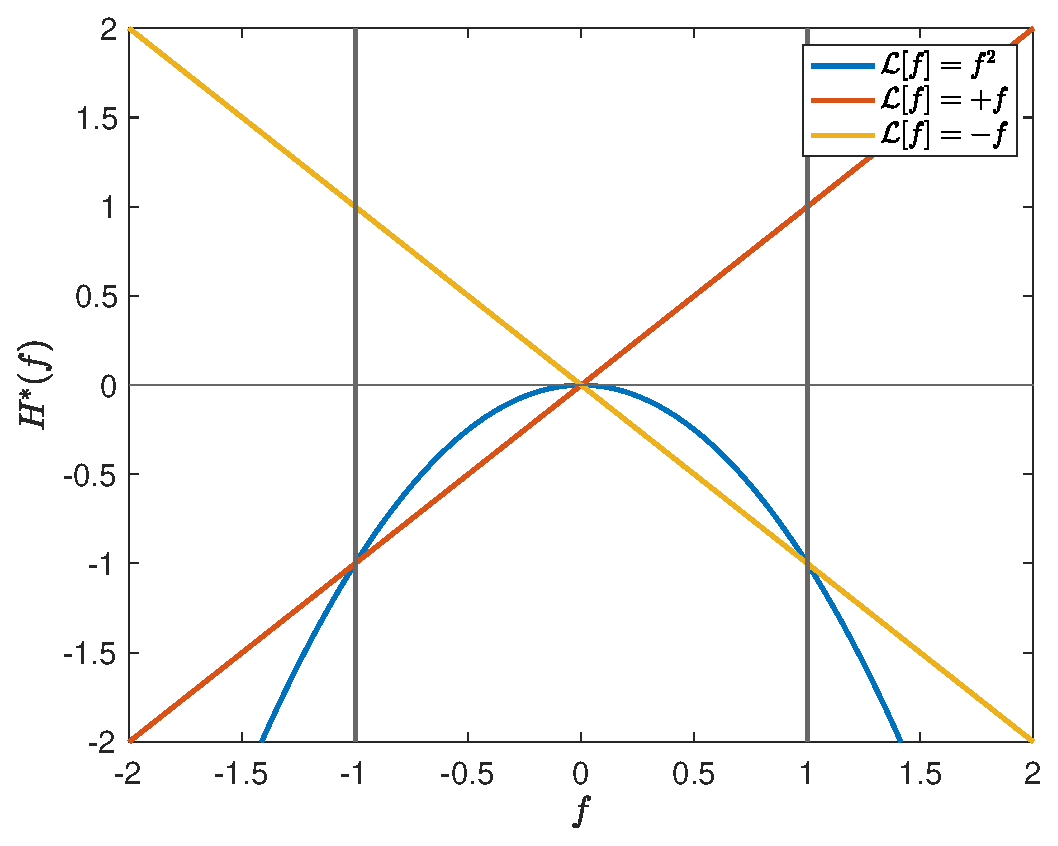
\includegraphics[scale=0.5]{img/bang-bang.eps}
    \caption{Ilustración sobre el comportamiento de la función $H^*(f)$ para distintos términos de penalización $\mathcal{L}[f]$}
\end{figure}


\subsection{OC SHE in two levels for symmetry of quarter-wave} 

Consideraremos un caso concreto del problema presentado en la sección anterior. Este es problema de selective harmonic elimination con simetría de cuarto de onda. Esta simetría implíca:
\begin{gather}
    f(\tau + \pi/2)   = f(\tau)    \ \ \tau \in (0,\pi/2)
\end{gather}

So this condition simplify the expressions of Fourier coefficients (\ref{an}) and (\ref{bn}), in this way:
\begin{align}
    a_i = & \  0 \ \ | \  \ \forall i \in \mathbb{Z} \\
    b_j = &  \frac{4}{\pi} \int_0^{\pi/2} f(\tau ) \sin(j\tau)d\tau \ | \ \forall j \ odd
\end{align}

In summary $f(\tau )$ can be written as follows:
\begin{gather}
    f(\tau ) = \sum_{j \ odd}^\infty  b_n \sin(j \tau) \\
    b_j = \frac{4}{\pi}\int_0^{\pi/2} f(\tau ) \sin(j\tau)d\tau \ \ | \ \ j \ odd \label{bn_odd}
\end{gather}


Now in this context, we can define a SHE problem as follows:


\begin{problem}\label{OCP_bn}
    Given  a set of odd numbers $\mathcal{E}_b$ with carinality $|\mathcal{E}_b| = N_b$ and given the target vector $\bm{b}_T  \in \mathbb{R}^{N_b}$, we search a wave form $f(\tau ) \ | \ \tau \in (0,\pi/2)$ such that $f(\tau)$ that minimize the following functional:

        \begin{gather}
        J[f(\tau)] = \Bigg[ || \bm{b}_T - \bm{\beta}(T)||^2 + \epsilon \int_0^{\pi/2} \mathcal{L}[f(\tau)] d\tau \Bigg] 
    \end{gather}

    where $ \bm{\beta}(\tau) \in \mathbb{R}^{N_b} \times [0,\pi/2] $, the $||.||$ is a euclidean norm and $\epsilon$ is a penalization parameter.
    \newline

    So, the optimal control problem can be written: 
    \begin{gather}
        \min_{|f(\tau) |<1} J[f(\tau)] \\
        \notag \text{suject to: } \\
        \notag \forall j \in \mathcal{E}_b \
        \begin{cases}
            \dot{\beta_j}(\tau) = (4/\pi) \sin(j\tau) f(\tau) & \tau \in [0,\pi/2]\label{dyn}\\
            \beta_j(0) = 0
        \end{cases} 
    \end{gather}
\end{problem}

En este caso el problema de control tiene el siguiente Hamiltoniano:
\begin{gather}
    H(f,\bm{p}_\beta,\tau) = -\epsilon  \mathcal{L}[f]+ 
    \frac{4f}{\pi} \Bigg[ 
        \sum_{j \in \mathcal{E}_b} p^\beta_j \sin(j\tau) 
    \Bigg]
\end{gather}

Podemos ver que el Hamiltoniano tiene la misma estructura que en el caso anterior, por lo que de la misma forma la elección de un término de penalización $\mathcal{L}[f]$ concavo nos produce un control óptimo $f^*$ \emph{bang-bang}.

\section{Experimentos numéricos}

To solve the optimal control problem (\ref{OCP_bn}), we use a direct method. 
If we consider a partition $\mathcal{P} = \{\tau_0,\tau_1,\dots,\tau_{T}\}$ of interval $[0,T]$ , we can represent a function $\{ f(\tau) \ | \ \tau \in [0,T]\}$ as a vector $\bm{f} \in \mathbb{R}^{T}$ where component $f_t = f(\tau_t)$. Then the optimal control problem (\ref{OCP_bn}) can be written as optimization problem with variable $\bm{f} \in \mathbb{R}^{T}$. This problem is a nonlinear programming, for this we use CasADi software to solve.


\subsection{OCP para SHE con simetría de media onda }

Dado una partición del intervalo $[0,\pi]$ podemos reformular el problema (\ref{OCP1}) como el siguiente problema en tiempo discreto:
\begin{problem}
    Dados dos conjuntos de números impares $\mathcal{E}_a$ and $\mathcal{E}_b$ con cardinalidades $|\mathcal{E}_a| = N_a$ y  $|\mathcal{E}_b| = N_b$ respectivamente , dados los vectores objetivos $\bm{a}_T  \in \mathbb{R}^{N_a}$ y $\bm{b}_T  \in \mathbb{R}^{N_b}$ y una  partition $\mathcal{P} = \{\tau_0,\tau_1,\dots,\tau_{T}\}$ of interval $[0,\pi]$. We search a vector $\bm{f} \in \mathbb{R}^{T}$ that minimize the following function:
    \begin{gather}
        \min_{\bm{f} \in \mathbb{R}^{T} } 
        \Bigg[ 
        || \bm{a}_T - \bm{\alpha}^{T}||^2 + 
        || \bm{b}_T - \bm{\beta}^{T}||^2 
        + \epsilon  \sum_{t=0}^{T-1} \mathcal{L}(f_{t}) \Delta\tau_t  \Bigg]  \\
        \notag \text{suject to: } \\
        \notag i \in \mathcal{E}_a \ \ 
        \begin{cases}
            \alpha_i^{t+1} = \alpha_i^{t} + \Delta \tau_t (2/\pi) \cos(i\tau_t) f_t \\
            \alpha_i^0 = 0
        \end{cases} \\
        \notag j \in \mathcal{E}_b \ \ 
        \begin{cases}
            \beta_j^{t+1} = \beta_j^{t} + \Delta \tau_t (2/\pi) \sin(j\tau_t) f_t \\
            \beta_j^0 = 0
        \end{cases} \\
        \notag |f_t| < 1 \ | \  \Delta \tau_t = \tau_{t+1} - \tau_{t} \ | \ \forall t \in \{1,\dots,T-1\}
    \end{gather}
\end{problem}

\subsubsection{Resultados numéricos para el problema SHE de dos niveles}

\subsubsection{Resultados numéricos para el problema SHE de tres niveles}

\subsection{OCP para SHE con simetría de cuarto de onda }

Dado una partición del intervalo $[0,\pi/2]$ podemos reformular el problema (\ref{OCP_bn}) como el siguiente problema en tiempo discreto:

\begin{problem}
    Given  a set of odd numbers $\mathcal{E}_b$ with carinality $|\mathcal{E}_b| = N_b$, given the target vector $\bm{b}_T  \in \mathbb{R}^{N_b}$ and  partition $\mathcal{P} = \{\tau_0,\tau_1,\dots,\tau_{T}\}$ of interval $[0,\pi/2]$. We search a vector $\bm{f} \in \mathbb{R}^{T}$ that minimize the following function:
    \begin{gather}
        \min_{\bm{f} \in \mathbb{R}^{T} } 
        \Bigg[ || \bm{b}_T - \bm{\beta}^{T}||^2 +
         \epsilon  \sum_{t=0}^{T-1} \mathcal{L}(f_{t}) \Delta\tau_t  \Bigg]  \\
        \notag \text{suject to: } \\
        \notag j \in \mathcal{E}_b \ \ 
        \begin{cases}
            \beta_j^{t+1} = \beta_j^{t} + \Delta \tau_t (4/\pi) \sin(j\tau_t) f_t \\
            \beta_j^0 = 0
        \end{cases} \\
        \notag |f_t| < 1 \  | \   \Delta \tau_t = \tau_{t+1} - \tau_{t} \ | \ \forall t \in \{1,\dots,T-1\}
    \end{gather}
\end{problem}


\subsubsection{SHE para dos niveles}

Para este ejemplo consideramos el siguiente conjunto de números impares: $\mathcal{E}_b = \{1,5,7,11,13\}$. Ademas consideramos el vector objetivo $\bm{b}_T = [m_a,0,0,0,0]$, donde  $m_a \in [0,1]$ es un parámetro. Compararemos la solución obenida mediante control óptimo con soluciones obtenidas en el problema (\ref{SHEp_clas}) (obtained via genetic algorithms). with three penalization terms: $\mathcal{L}(f) = -f$, $\mathcal{L}(f) = +f$ and $\mathcal{L}(f) = -f^2$ obtained by direct method with uniform partition of interval $[0,\pi/2]$ with $T=400$ and penalization parameter $\epsilon = 10^{-5}$. To obtain the solutions of problem (\ref{SHEp_clas}) we considered the number of switching angles $M=5$. 

Mostramos en la figura (\ref{fig:error_solutions}) los errores para tres soluciones obtenidas mediante algoritmos genéticos del problema (\ref{SHEp_clas}) y tres soluciones obtenidas mediante control óptimo con los distintos términos de penalización.  Esto nos asegura que el orden de magnitud de las soluciones obtenidas son del mismo orden. Además podemos ver en la figura (\ref{fig:solutions}) que el control óptimo con los términos $\mathcal{L}(f) = -f$ y $\mathcal{L}(f) = +f$ recuperar dos soluciones obtenido del problema (\ref{SHEp_clas}). Mientras que el problema de control con el término $\mathcal{L}(f) = f^2$ es solución del problema pero no presenta continuidad con respecto $m_a$.
 
\begin{figure}[!ht] 
        \centering
        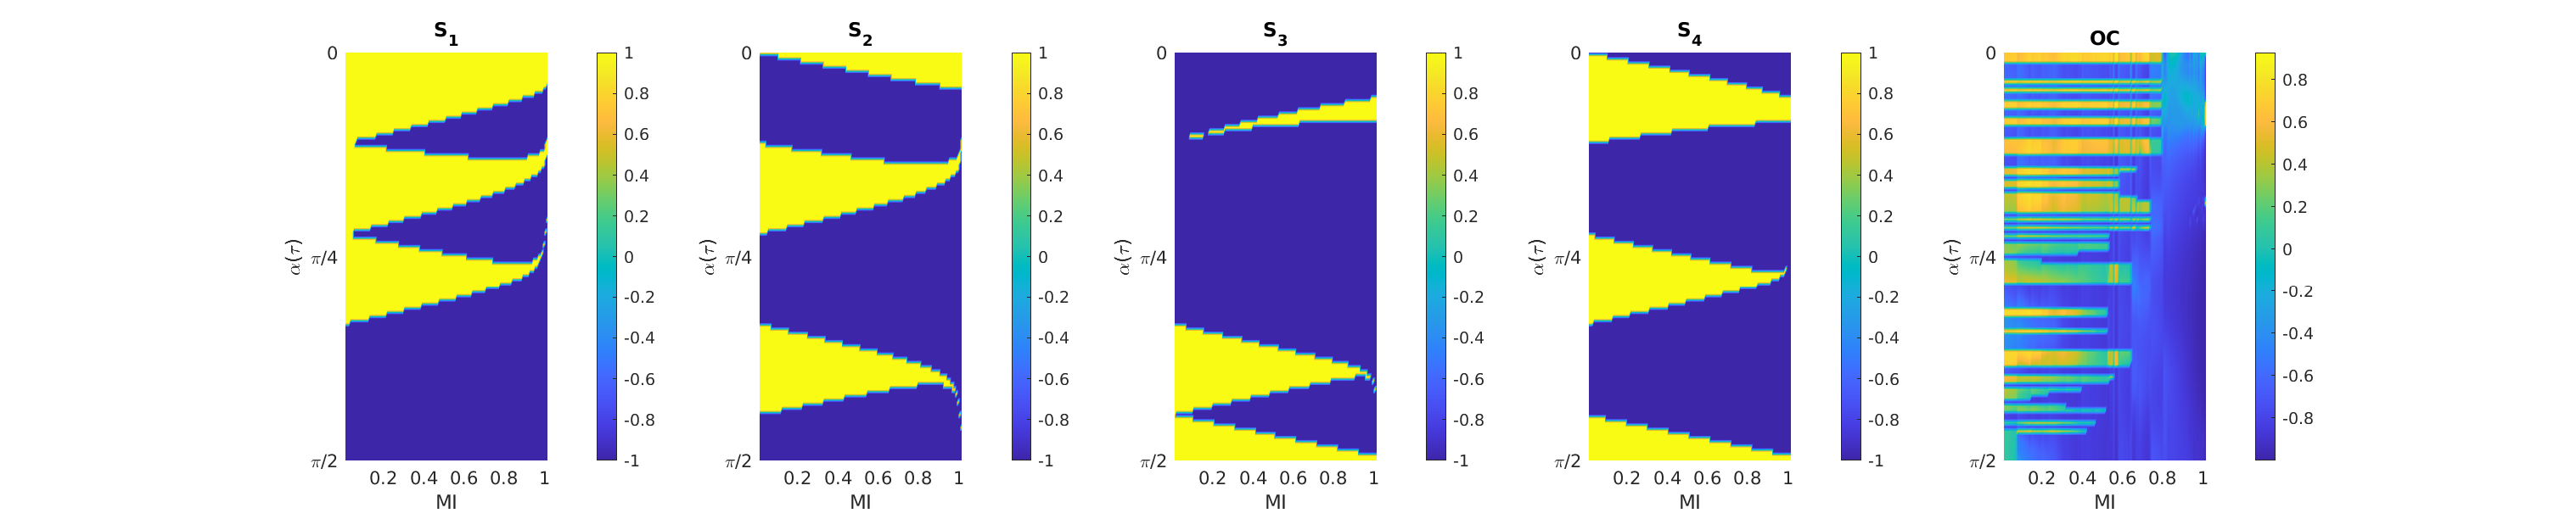
\includegraphics[scale=0.5]{img/EX01_surf.eps}
        \caption{Comparison of solutions for different values of $m_a$. Solutions $S_1$, $S_2$, $S_3$ correspond to problem (\ref{SHEp_clas}) where the number of switching angles is prefixed, while $OC$ solution correspond to optimal control problem with different $\mathcal{L}(f)$. }
        \label{fig:solutions}
    \end{figure}


 
\begin{figure}
    \centering
    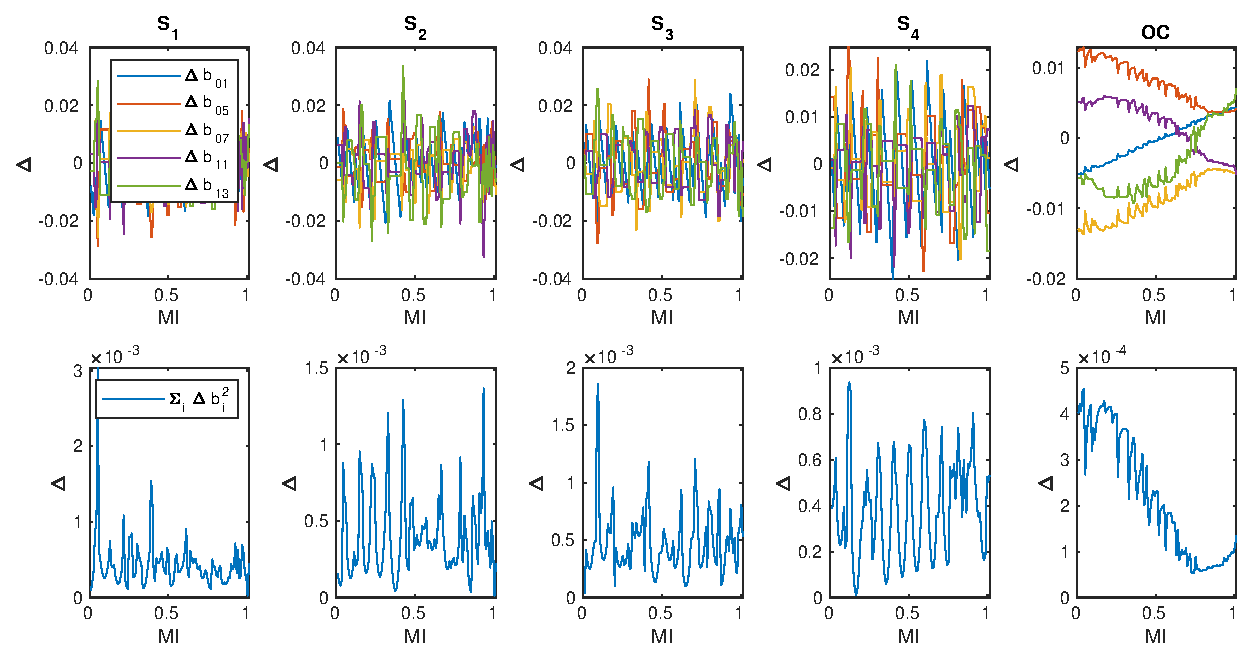
\includegraphics[scale=0.6]{img/EX01.eps}
    \caption{The order of magnitud of the square of euclidean distantes to target is the same for all solutions of figure (\ref{fig:solutions})}
    \label{fig:error_solutions}
\end{figure}

\subsubsection{SHE para tres niveles}

Podemos ver que en el caso en el que el control $f(\tau)$ solo pueda tomar valores entre $[0,1]$ obtenemos señales que pueden tomar tres niveles en el intervalo $[0,2\pi]$ gracias a la simetría de cuarto de onda. Si resolvemos el problema de control óptimo pero esta vez cambiando las restricciones $|f(\tau)|<1$ por $\{0<f(\tau)<1\}$. Se ha realizado el mismo procedimiento que en el caso anterior, obteniendo soluciones para los mismo términos de penalización.

\begin{figure}
    \centering
    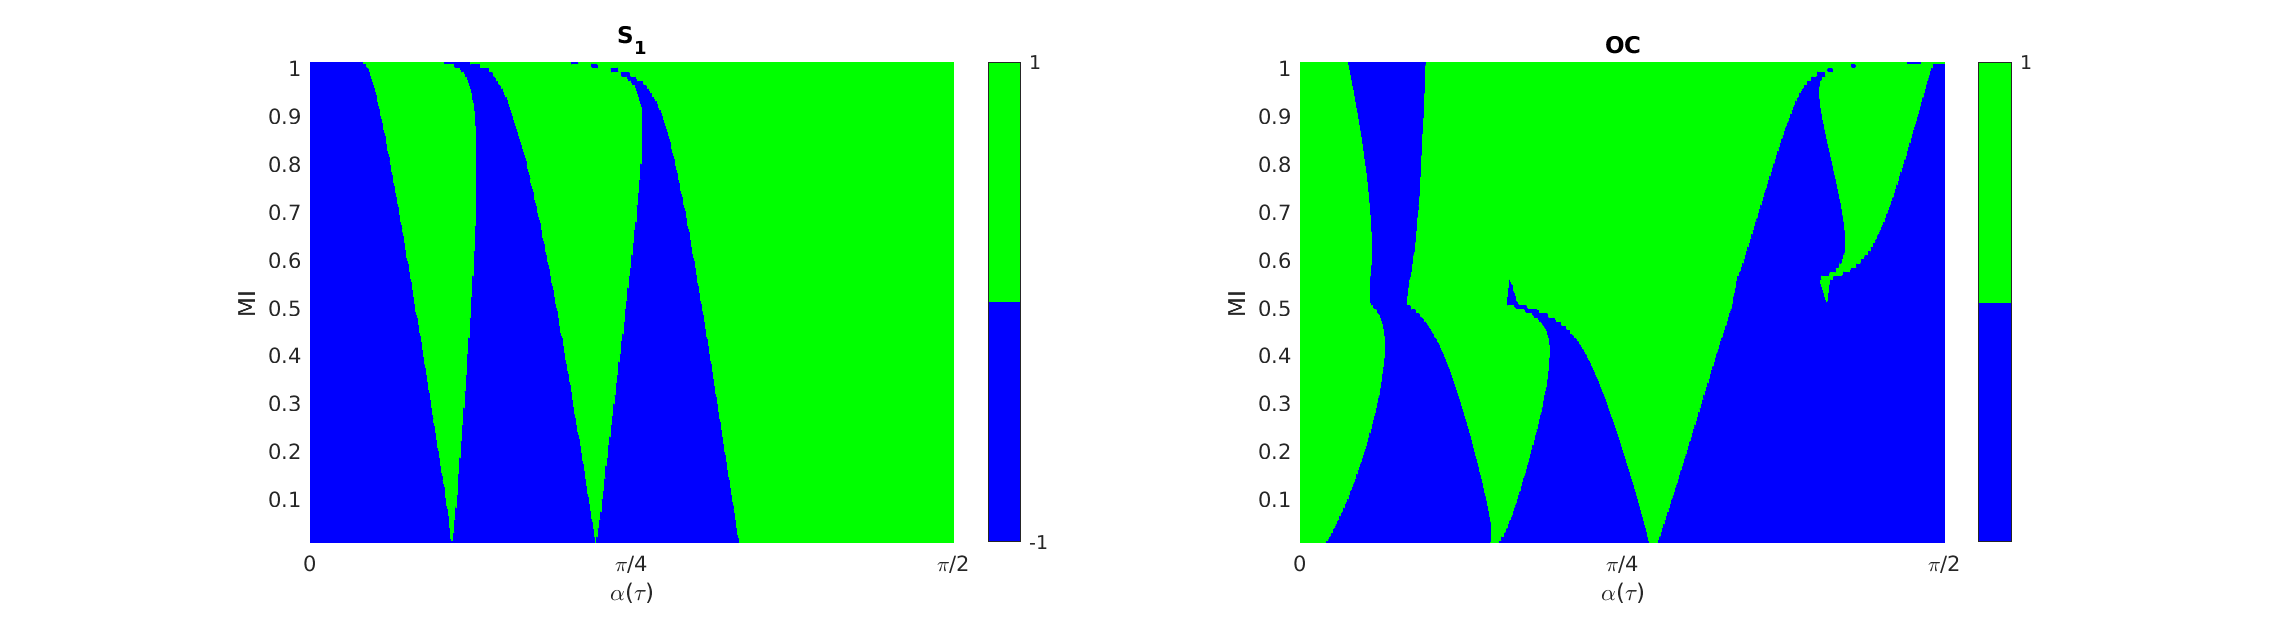
\includegraphics[scale=0.45]{img/EX01_surf_3LVL.eps}
    \caption{Soluciones para un control  con restriciones $0 \leq f\leq 1$ para obtener soluciones de tres niveles.}
\end{figure}

\begin{figure}
    \centering
    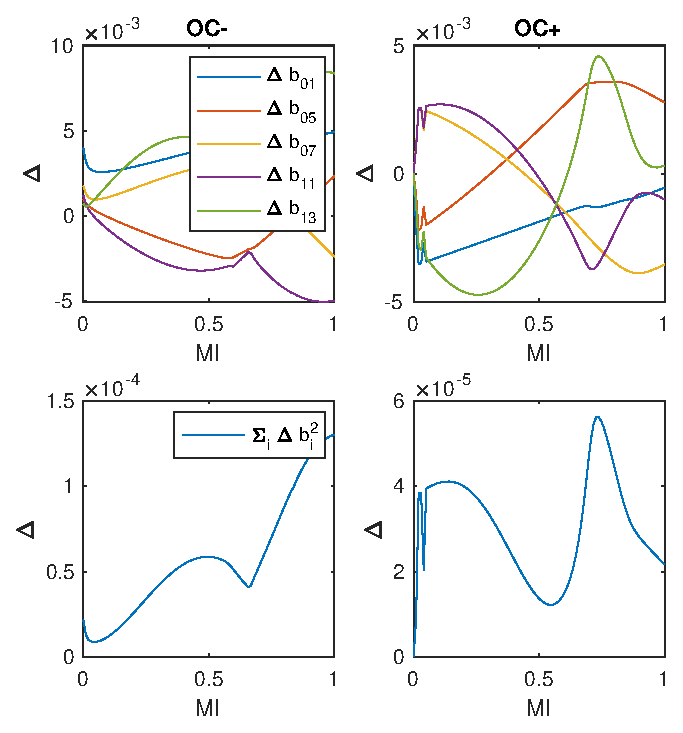
\includegraphics[scale=0.7]{img/EX01_3LVL.eps}
    \caption{Errors of solution in three level solutions}
\end{figure}
 
  
\newpage
\part{Feedback Optimal Control}
\section{SHE with quarter-wave symmetry as dynamic programming problem}

Con el fin de encontrar la solución al problema para distintos targets $\bm{a}_T$ y $\bm{b}_T$ consideraremos el cambio de variable $\bm{\beta}'(\tau) = \bm{\beta}(\tau) - \bm{b}_T$. De manera que, podemos plantear un problema de control donde el estado inicial el target $\bm{b}_T$ y cuyo objetivo es llevar el sistema al origen de coordenadas.
\begin{problem}
    Given  $\bm{b}_T  \in \mathbb{R}^{n_b}$, we define a cost functional in this way: 
        \begin{gather}
        J[f(\tau)] =  \frac{1}{2}|| \bm{\beta}(T)||^2  
    \end{gather}


    So, the optimization problem can be written: 
    \begin{gather}
        \min_{f \in \{-1,1\} } J[f(\tau)]) \\
        \notag \text{suject to: } \\
        \notag \forall j \in \mathcal{E}_b
        \begin{cases}
            \dot{\beta_j(\tau)} =  - (4/\pi) \sin(j\tau) f(\tau) & \tau \in [0,\pi/2]\label{dyn}\\
            \beta_j(0) = b_T^j
        \end{cases} \\
    \end{gather}
    
\end{problem}

En este caso, no consideraremos ningún término de penalización de manera que la solución del problema sea compatible con todas las posibles soluciones.

Tomamo un discretización $\{\tau_0,\tau_1,\dots,\tau_{N_t} \}$ del intervalo $[0,\pi/2]$. Entonces podemos discretizar el problema anterior:

\begin{problem}
    Given  $\bm{b}_T  \in \mathbb{R}^{n_b}$,  the optimization problem can be written: 
    \begin{gather}
        \min_{\bm{f} \in \mathbb{R}^{N_t} } \frac{1}{2}||\bm{\beta}^{N_t}||^2 \\
        \text{suject to: }
        \begin{cases}
            \beta_n^{i+1} = \beta_n^{i} - \Delta \tau (4/\pi) \sin(n\tau_i) f_\tau & \tau \in [0,\pi/2]\label{dyn}\\
            \beta_n^0 = b_T^n
        \end{cases} \\
        \notag \forall n \in \{1,3,5,\dots,N/2 \}
    \end{gather}

\end{problem}

\subsection{Dynamic programming}

Función valor 

\begin{gather}
    v_t(\bm{b}_T) =  \min_{\bm{f} \in \mathbb{R}^{N_t-t} } \frac{1}{2}||\bm{\beta}^{t}||^2 \\
    \text{suject to: }
    \begin{cases}
        \beta_n^{i+1} = \beta_n^{i} - \Delta \tau (4/\pi) \sin(n\tau_i) f_\tau & \tau \in [0,\pi/2]\label{dyn}\\
        \beta_n^0 = b_T^n
    \end{cases} \\
    \notag \forall n \in \{1,3,5,\dots,N/2 \}
\end{gather}




Entonces la función valor de estado cumple la ecuación de Bellman, que en este caso se puede escribir como:
\begin{gather}\label{BellmanEquationOptimo}
    v_t(\bm{\beta}^t) = \min_{f \in \{ -1,1 \}}  v_{t+1}(\bm{\beta}^{t+1})  \\
    v^{N_t}(\bm{\beta}^{N_t}) =  \frac{1}{2}|| \bm{\beta}^{N_t}||^2
\end{gather}

La función $v_t(\bm{\beta}^t)$ representa el mejor coste que se puede alcanzar desde el estado $\bm{\beta}^t$ en $(N_t-t)$ pasos. Es por ello que en $t=Nt$ el mejor coste que se puede alcanzar desde el punto $\bm{\beta}^t$ es el valor del coste final $\frac{1}{2} || \bm{\beta}^{N_t}||^2$


Luego el control óptimo se puede calcular mediante la siguiente expresión 

\begin{gather}
    f^*(\tau,\bm{\beta}_t) = \min_{f \in \{ -1,1\}} v_t(\bm{\beta}_t)
\end{gather}

% \begin{algorithm}[!ht]
%     \caption{\emph{Value Iteration}}\label{ValueIteration}
%     \begin{algorithmic}[1]
%         \Procedure{Value-Iteration}{$\mathcal{V}^*,tol$}
%         \State $k \gets 0$
%         \State $\mathcal{V}_k\gets \mathcal{V}^*$
%         \While{$error\leq tol$}
%             \State $k \gets k + 1$
%             \For{$\forall s \in \Ss$}
%                 \State $\mathcal{V}_k(s)\gets \mathcal{T}_v\mathcal{V}_{k-1}(s)$
%             \EndFor
%             \State $error \gets || \mathcal{V}_k - \mathcal{V}_{k-1}||_\infty$
%         \EndWhile
%         \State $\displaystyle \pi_k^*(s) = \arg \max_{a'\in \As} \bigg[ r(s,a') + \gamma \sum_{s'}p(s'|s,a') v_*(s')
%         \bigg]$
%         \State \textbf{return}: [$\mathcal{V}_k(s)$,$\pi_k^*(s)$]
%         \EndProcedure
%     \end{algorithmic}
% \end{algorithm}

\newpage
\appendix


\section{Other}


\begin{gather}
    \int_0^{\pi/2} ||f(\tau) ||^2 d\tau = \pi/2
\end{gather}

\begin{gather}
    \int_0^{\pi/2} ||f(\tau) ||^2 d\tau = \pi/2
    \int_0^{\pi/2} || \sum_{n \ odd}^\infty b_n \sin(n\tau) ||^2 d\tau = \pi/2\\
    \int_0^{\pi/2}  \sum_{n,n' \ odd}^\infty b_n b_n' \sin(n\tau)\sin(n'\tau)  d\tau = \pi/2\\
    \sum_{n,n' \ odd}^\infty b_n b_n' \int_0^{\pi/2}\sin(n\tau)\sin(n'\tau)  d\tau = \pi/2 \\
    ?? \\
    \frac{\pi}{4} \sum_{n \ odd}^\infty b_n^2  = \pi/2 \\
    \sum_{n \ odd}^\infty b_n^2  = 2 
\end{gather}

 
\bibliographystyle{apalike}
\bibliography{bib}

\end{document}